\documentclass{report}
\usepackage[utf8]{inputenc}
\title{DeSem}
\author{Rémy Macherel}
\date{\today}
\usepackage[utf8]{inputenc}
\usepackage[T1]{fontenc}
\usepackage[english]{babel}
\usepackage{hyperref}
\hypersetup{
    colorlinks=true,
    linkcolor=blue,
    filecolor=blue,      
    urlcolor=blue,
    pdftitle={DeSEm project report},
    pdfpagemode=FullScreen,
    }
\usepackage{lmodern}
\usepackage{url}
\usepackage{wrapfig}
\usepackage{graphicx,subfigure}
\usepackage{textcomp}
\usepackage{float}
\usepackage{lastpage}
\usepackage{wrapfig}
\usepackage[top=3cm, bottom=3.5cm, left=3cm, right=3cm]{geometry}
\usepackage{fancyhdr}
\usepackage{lastpage}
% \usepackage[dvipsnames]{xcolor}
\usepackage{titlesec}
\usepackage{setspace}
%\usepackage{minted}
\usepackage{multirow}
\usepackage[export]{adjustbox}
\usepackage{subfigure}
\usepackage{titlesec}
\usepackage{setspace}
\usepackage{tikz}
\usepackage{tabto}
\usepackage{ragged2e}
\usepackage{pdfpages}
\usepackage[sorting = none]{biblatex}
\usepackage{csquotes}
\usepackage{enumitem}
\usepackage{caption}
\usepackage{amsmath}

\setcounter{tocdepth}{3}
\setcounter{secnumdepth}{3}
\pagestyle{fancy}
\fancypagestyle{plain}{}
\setlength{\headheight}{55pt}
\renewcommand\headrulewidth{1pt}
\fancyhead[L]{
\includegraphics[scale = 0.2]{./Images/Base/LogoHESSO.png}}
\fancyhead[R]{
\includegraphics[scale = 0.3]{./Images/Base/LogoMSE.png}}
\fancyhead[C]{DeSenet Laboratory}
\fancyfoot[L]{Page \thepage ~sur \pageref{LastPage}}
\fancyfoot[C]{Rémy Macherel}
% \fancyfoot[R]{Yverdon-les-Bains, le \today}
\titleformat{\chapter}[hang]
  {\normalfont\LARGE\bfseries}
  {\thechapter.}{1em}{\LARGE}
  \titlespacing*{\chapter}{0pt}{10pt}{10pt}


\makeatletter
\let\mytitle\@title
\let\myauthor\@author
\let\mydate\@date
\makeatother


\begin{document}
\begin{titlepage}
% \hspace{0pt}
% \vfill
 \line(1,0){420}
	\begin{center}
	\huge{\textbf{\mytitle}} \\
	\huge{DeSenet laboratory report}\\
	\LARGE{\myauthor} \\
	\LARGE{\mydate}
 \line(1,0){420}
 \end{center}
\textbf{\underline{Authors :}} \hfill \textbf{\underline{Teacher : }}\newline
Macherel Rémy \hfill Rieder Medard\newline
\hfill Sterren Thomas
\end{titlepage}
\chapter{Introduction}
Dans le cadre du cours MA-DeSem, il nous a été demandé de réaliser le protocole DeseNET sur un système de type STM32 Nucleo. Les spécifications du protocole de communication ont été fournies pour ce travail.\newline
La structure de base du projet fût fournie et nous avons du apporter les modifications nécessaires au bon fonctionnement du protocole.
\chapter{Modifications du code}
\begin{figure}[H]
    \centering
    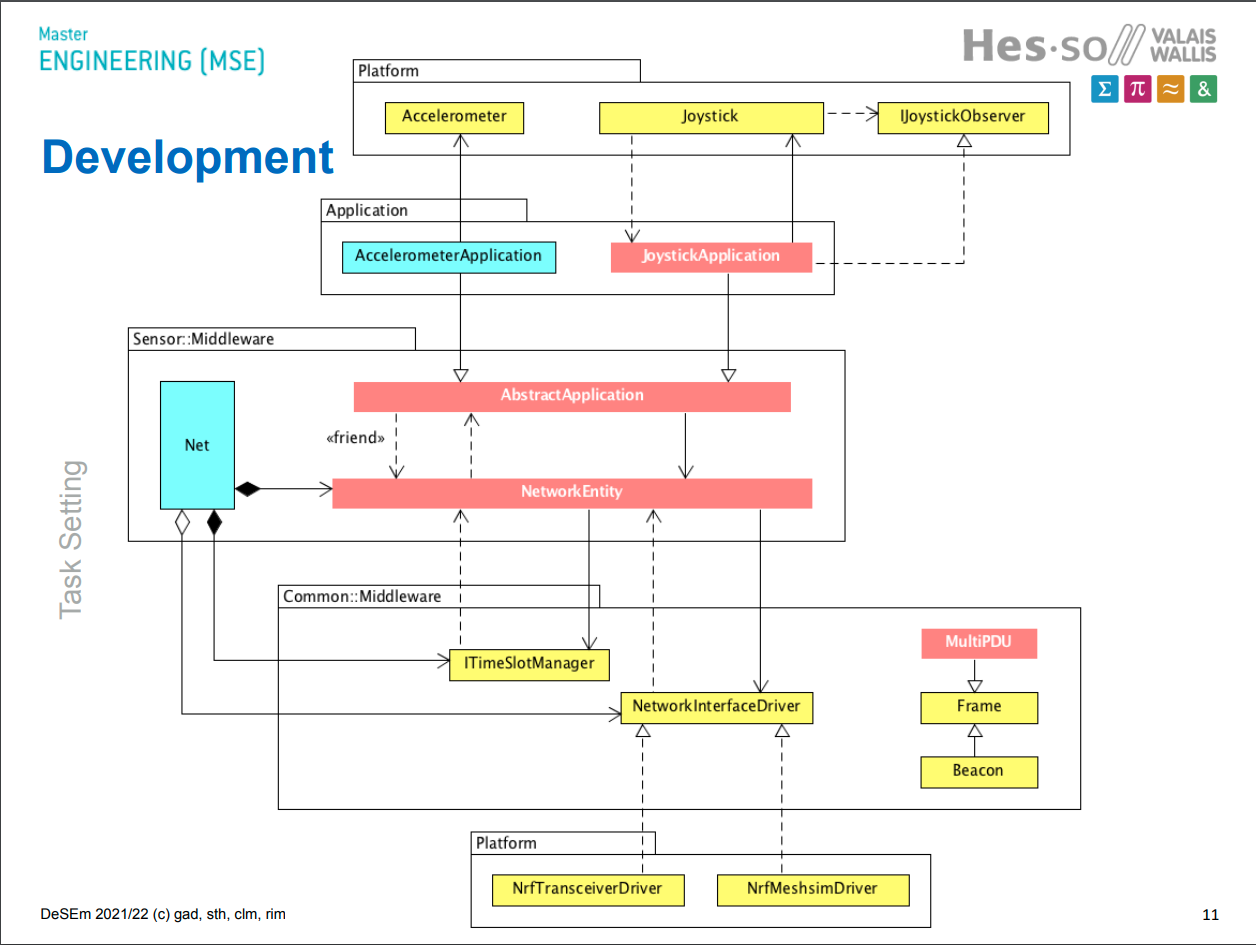
\includegraphics[width= 0.8\textwidth]{Images/ClassesToImplement.png}
    \caption{Aperçu des modifications à apporter}
    \label{fig:ClassesToModify}
\end{figure}
La figure suivante nous a été présentée afin d'illustrer les classes que nous devions compléter/créer. Les classes à créer sont les suivantes :
\begin{enumerate}
\item JoystickApplication (.h et .cpp)
\item MPDU (.h et .cpp)
\end{enumerate}
Alors que les classes à compléter sont :
\begin{enumerate}
\item AbstractApplication (.h et .cpp)
\item NetworkEntity (.h et .cpp)
\end{enumerate}
D'autres fichiers ont cependant également été modifiés comme par exemple Factory.cpp afin d'y ajouter l'initialisation du Joystick ainsi que le setObserver().\newline

\chapter{Diagrammes UML des classes implémentées}

\end{document}